\chapter{Propostas}
\label{cha:propostas}

Esse capítulo tem como base as oportunidades, fraquezas e ameaças do programa Ocean levantados no capítulo anterior, e tem como objetivo definir e criar uma proposta de desenvolvimento para um deles. Embora todos os pontos sejam levados até a gestão PRO/Samsung, foram realizado um critério de priorização de forma a selecionar os mais relevantes para serem desenvolvidos.

\section{Análise das oportunidades, fraquezas e ameaças}

De forma a facilitar a priorização dos pontos a serem trabalhados, as oportunidades, fraquezas e ameaças foram agrupadas em 4 categorias, explicadas a seguir: 

\begin{description}

\item[Pontos "passivos"] - Alguns pontos levantados não geram nenhuma ação a ser realizada por parte da gestão do laboratório, pois a gestão já permite o seu desenvolvimento, só faltando oportunidades ou resultados que aparecerão com o tempo. Entre esses pontos estão "Utilização do laboratório para a pós-graduação, na geração de pesquisas", "Maior utilização do laboratório em aulas do departamento", "Expansão dos projetos e parcerias (NEU) além dos cursos intensivos" e "Instituições de aceleração de empresas não-gratuitas podem tentar entrar na universidade". Os três primeiros pontos não apresentam nenhuma barreira para se desenvolverem naturalmente, e são fatores que a gestão acompanhará de perto. O último é considerado pela gestão improvável de acontecer pois com o aumento de instituições de aceleração oferecendo cursos bons gratuitos dentro da universidade, as instituições pagas têm menos incentivo para querer entrar na universidade.

\begin{figure}[H]
\caption{Pontos Passivos}
\centerline{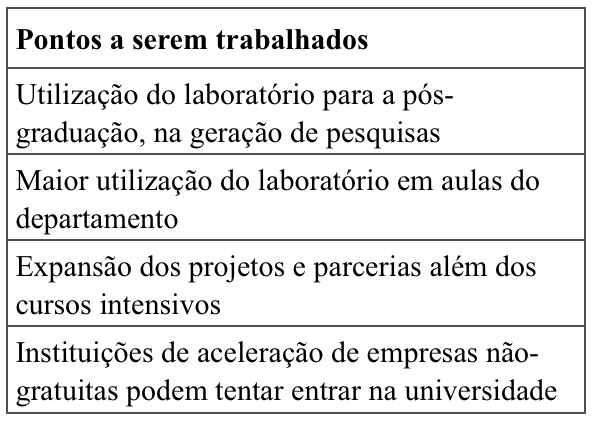
\includegraphics[scale=0.75]{img/pontosselecionadospassivos}}
\label{fig:pontosselecionadospassivos}
\caption* {Fonte: Elaborado pelo próprio autor}
\end{figure}

\item[Pontos levantados pelos cursistas] - Em relação aos pontos levantados sobre \textit{feedbacks} dos cursistas, será elaborado um relatório executivo com menor teor acadêmico porém mais detalhes diante das análises realizadas. Em relação aos cursos básicos, poderá será feita uma segmentação dos \textit{feedbacks} por ano de realização do questionário ou por tipo de curso dado pelo laboratório. Já para os cursos intensivos, poderão ser explorados os pontos levantados do ponto de vista de cada grupo, incluindo a identificação de 'frases de efeito' que poderiam ser utilizadas em um material de divulgação do curso. Não obstante, como esses pontos devem ser trabalhados quase que exclusivamente pela gestão da Samsung, serão levantadas questões a respeito de como desenvolver esses pontos, porém eles apresentam pouca prioridade para os fins deste trabalho.

\begin{figure}[H]
\caption{Pontos levantados pelos cursistas}
\centerline{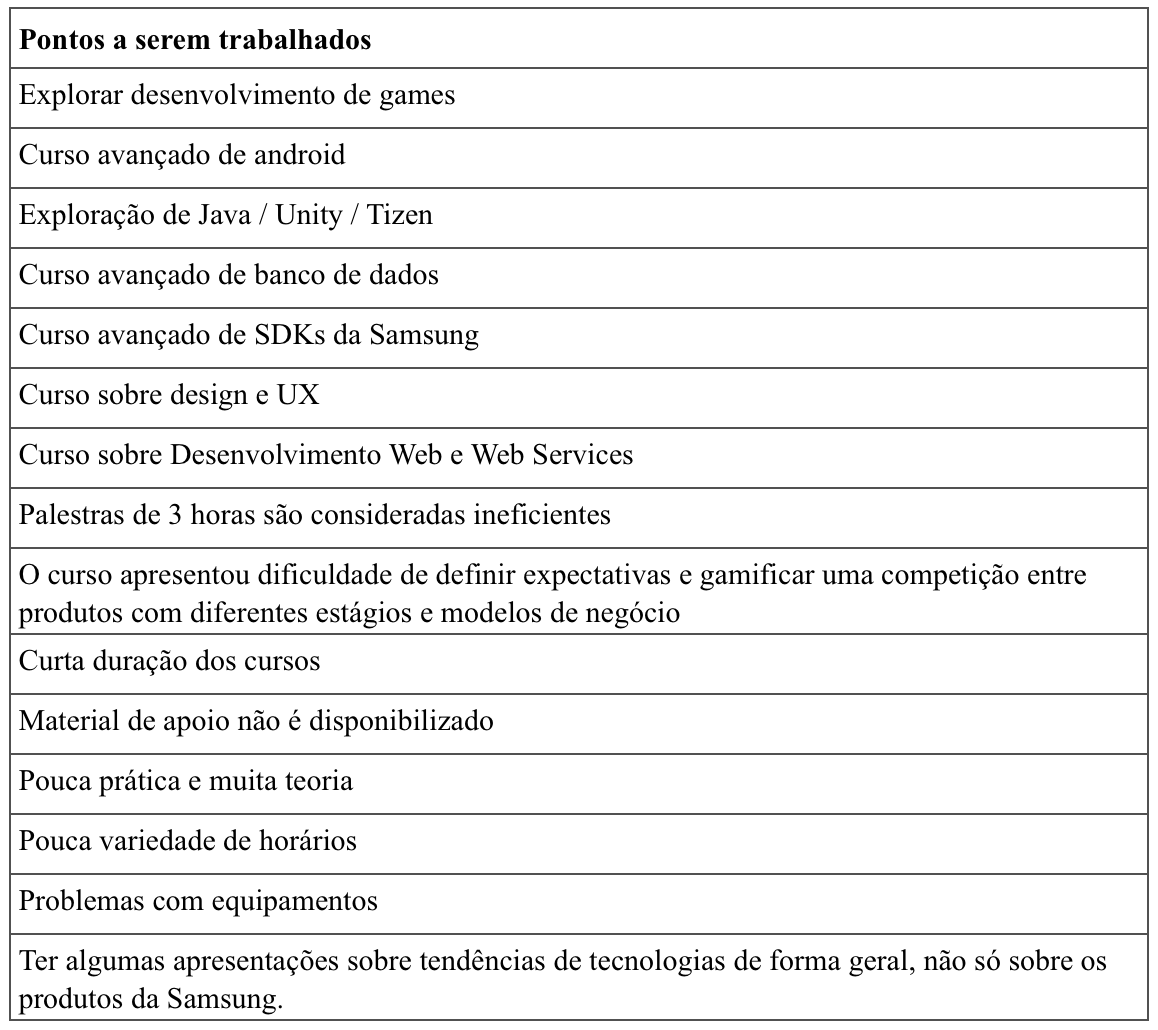
\includegraphics[scale=0.75]{img/pontosselecionadoscursistas}}
\label{fig:pontosselecionadoscursistas}
\caption* {Fonte: Elaborado pelo próprio autor}
\end{figure}

\item[Pontos considerados operacionais] - Os pontos operacionais são aqueles que podem ser corrigidos com alguma ação a ser tomada sem a necessidade de tomar algum decisão considerada estratégica pela gestão. Dentro desses pontos estão "Falta de conhecimento sobre os programas do laboratório", "Falta de instruções sobre o processo de utilização" e "Falta de agenda pública com os compromissos do Ocean". São pontos relevantes, e a gestão deverá fazer algo a respeito deles para maximizar o uso do laboratório pelos alunos.

\begin{figure}[H]
\caption{Pontos operacionais}
\centerline{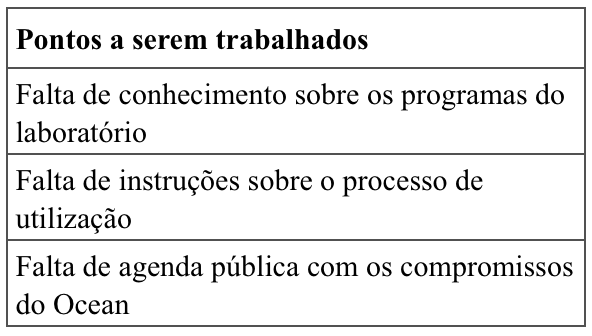
\includegraphics[scale=0.75]{img/pontosselecionadosoperacionais}}
\label{fig:pontosselecionadosoperacionais}
\caption* {Fonte: Elaborado pelo próprio autor}
\end{figure}

\item[Pontos estratégicos] - Os pontos considerados mais estratégicos são aqueles que podem ser desenvolvidos e transformados em projetos de curto, médio ou longo prazo, e têm potencial de trazer um impacto muito positivo para o Ocean.

\begin{figure}[H]
\caption{Pontos estratégicos}
\centerline{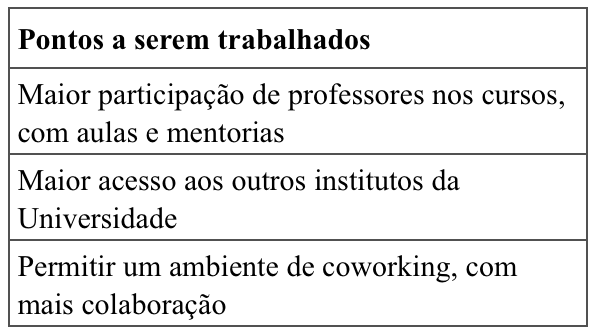
\includegraphics[scale=0.75]{img/pontosselecionadosestrategicos}}
\label{fig:pontosselecionadosestrategicos}
\caption* {Fonte: Elaborado pelo próprio autor}
\end{figure}

\end{description}

Definidas as categorias, foram definidos níveis de priorização para cada uma, juntamente com a gestão do laboratório Ocean. Foram atribuídas as notas 1, 3, 5 e 7 para as categorias, sendo a nota 1 os pontos prioritários e o 7 o de menor prioridade.


\begin{figure}[H]
\caption{Priorização de pontos}
\centerline{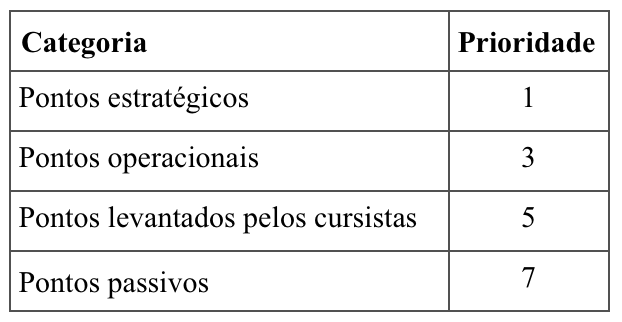
\includegraphics[scale=0.75]{img/priorizacao}}
\label{fig:priorizacao}
\caption* {Fonte: Elaborado pelo próprio autor}
\end{figure}

\section{Desenvolvimento dos pontos prioritários}

Cada um dos pontos 

Os dois primeiros pontos em questão estão sendo avaliados pelo departamento, pois envolvem uma remuneração extra para os professores participarem nesses cursos e uma maior divulgação do laboratório por parte de todos os \textit{stakeholders}, principalmente o NEU e o PRO. Portanto juntamente à gestão do PRO e da Samsung, foi definido que seria desenvolvido o terceiro ponto mencionado, \textbf{"Permitir um ambiente de \textit{coworking}, com mais colaboração"}, pois além de ser uma questão estratégica para o laboratório, ele pode evitar o problema de o laboratório se tornar uma biblioteca ou uma pró-aluno.
